\begin{frame}
  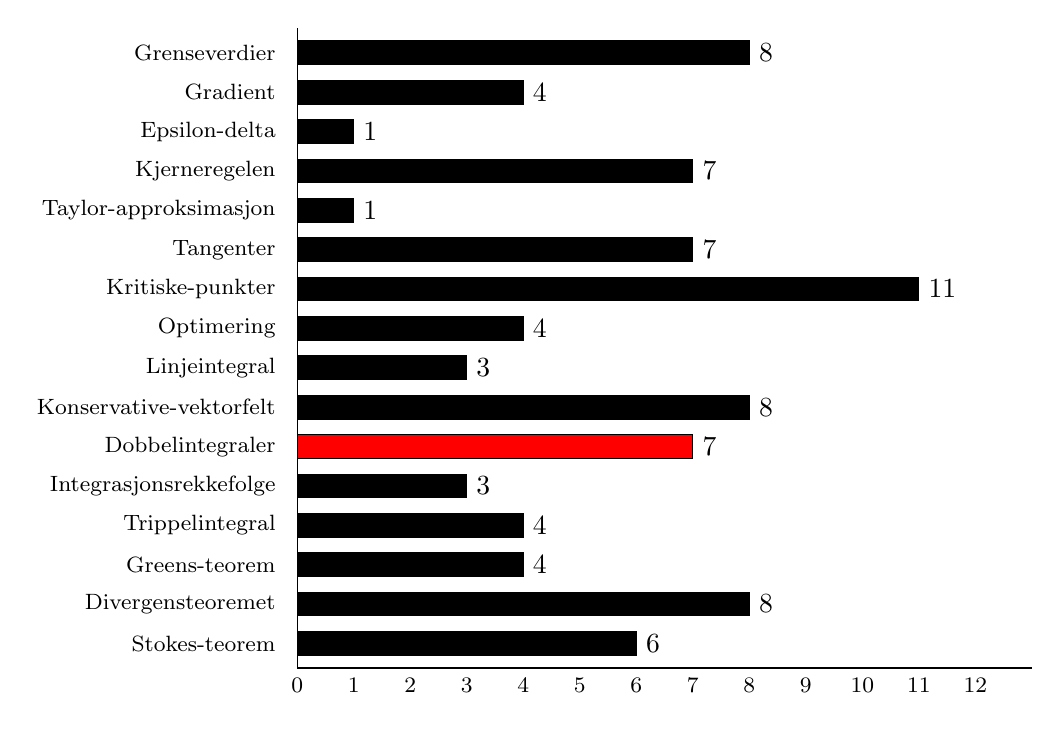
\begin{tikzpicture}
    \begin{axis}[ xbar=0pt, /pgf/bar shift=0pt, legend style={ legend columns=4,
        at={(xticklabel cs:0.5)}, anchor=north, draw=none }, ytick={0,...,15},
      ytick style={draw=none},% <- added
      axis y line*=none, axis x line*=bottom, tick label
      style={font=\footnotesize}, legend style={font=\footnotesize}, label
      style={font=\footnotesize}, xtick style={draw=none},% <- added
      xtick={0,1,...,12}, width=.9\textwidth, bar width=3mm, y dir = reverse,
      xmin=0, xmax=13, area legend,
      y=5mm, enlarge y limits={abs=0.625},
      style={text=black}, every axis plot/.append style={fill},
      nodes near coords, nodes near coords,
      yticklabels={%
        {\topicref{Grenseverdier}},
        {\topicref{Gradient}},
        {\topicref{Epsilon-delta}},
        {\topicref{Kjerneregelen}},
        {\topicref{Taylor-approksimasjon}},
        {\topicref{Tangenter}},
        {\topicref{Kritiske-punkter}},
        {\topicref{Optimering}},
        {\topicref{Linjeintegral}},
        {\topicref{Konservative-vektorfelt}},
        {\topicref{Dobbelintegraler}},
        {\topicref{Integrasjonsrekkefolge}},
        {\topicref{Trippelintegral}},
        {\topicref{Greens-teorem}},
        {\topicref{Divergensteoremet}},
        {\topicref{Stokes-teorem}}}]
      \addplot[fill=black] coordinates {(8,0)};
      \addplot[fill=black] coordinates {(4,1)};
      \addplot[fill=black] coordinates {(1,2)};
      \addplot[fill=black] coordinates {(7,3)};
      \addplot[fill=black] coordinates {(1,4)};
      \addplot[fill=black] coordinates {(7,5)};
      \addplot[fill=black] coordinates {(11,6)};
      \addplot[fill=black] coordinates {(4,7)};
      \addplot[fill=black] coordinates {(3,8)};
      \addplot[fill=black] coordinates {(8,9)};
      \addplot[fill=red] coordinates {(7,10)};
      \addplot[fill=black] coordinates {(3,11)};
      \addplot[fill=black] coordinates {(4,12)};
      \addplot[fill=black] coordinates {(4,13)};
      \addplot[fill=black] coordinates {(8,14)};
      \addplot[fill=black] coordinates {(6,15)};
    \end{axis}
  \end{tikzpicture}
\end{frame}

\begin{frame}
  \subsection{Dobbelintegraler}\label{subsec:Dobbelintegraler}
  \frametitle{Dobbelintegraler}
  \begin{enumerate}
    \item Integralet av en odde funksjon omkring et symmetrisk området er null
      \begin{equation*}
        \int_{-a}^{a} \only<1>{x}\only<2->{f(x)} \dx = 0
      \end{equation*}
      %
      \visible<2>{Hvor $f(-x) = -f(x)$.}
    \item Dersom integralet inneholder $x^2 + y^2$ bytt til polarkoordinater
      \begin{equation*}
        x^2 + y^2 = r^2 \quad x = r \cos \theta, y = r \sin \theta \quad \dx \dy = r \dd r \dT 
      \end{equation*}
      
  \end{enumerate}
\end{frame}

\begin{frame}
  \begin{oppgave}{V2017, Oppgave 4} Beregn dobbelintegralet $\displaystyle\iint_{D}
    3 + x^3\dd(x,y)$ der $D$ er gitt ved $x^2 + y^2 \leq a^2$.
  \end{oppgave}
  \only<1->{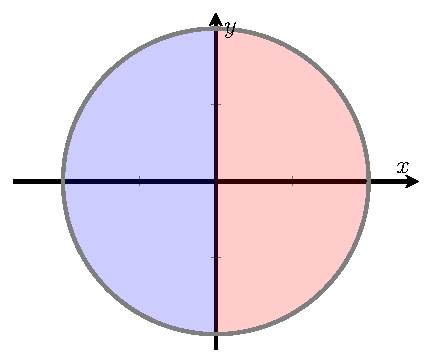
\includegraphics[width=0.4\textwidth]{../img/dobbel-polar-xy}}
  \only<2->{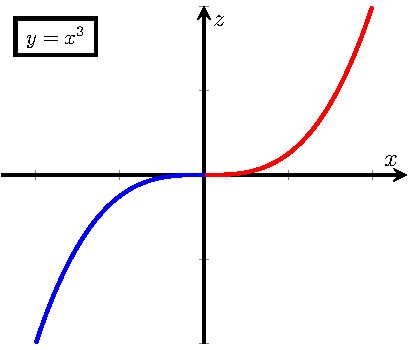
\includegraphics[width=0.4\textwidth]{../img/dobbel-polar-zx}} 
  \only<3>{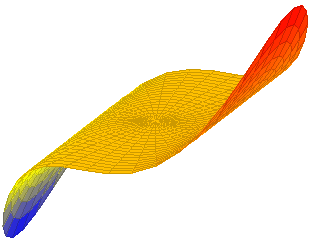
\includegraphics[width=0.3\textwidth]{../img/dobbel-polar3d}}
  \only<4->{%
  \begin{equation*}
    \iint_{D} 3 + x^3\dd(x,y)
    \visible<5->{
      \only<6>{= 3 \iint_{D} \dd(x,y) + \iint_D x^3 \dd(x,y)}
      \only<7->{= 3 \underbrace{\iint_{D} \dd(x,y)}_{\pi a^2} + \underbrace{\iint_D x^3 \dd(x,y)}_{0}
    = 3 \pi a^2}}
  \end{equation*}}
\end{frame}

\begin{frame}
  \begin{oppgave}{V2017, Oppgave 4} Beregn dobbelintegralet $\displaystyle\iint_{D}
    3 + x^3\dd(x,y)$ der $D$ er gitt ved $x^2 + y^2 \leq a^2$.
  \end{oppgave}
  Bytter direkte til polarkoordinater
  %
  \begin{align*}
    \iint_D 3 + x^3 \dd(x,y)
    & = \int_0^{2\pi} \int_0^{a} (3 + (r \cos \theta)^3) r \dd r \dT \\
    & = \int_0^{2\pi} \left[ \only<1>{\int 3r + r^4(\cos \theta) \dd r}\only<2->{\frac{3}{2}r^2 + \frac{r^5}{5} (\cos \theta)^3} \right]_0^a  \dT \visible<3->{\\
    & = \int_0^{2\pi} \frac{3}{2}a^2 + \frac{a^5}{5} (\cos \theta)^3 \dT \visible<4->{\\
    & = 3\pi a^2 + \frac{a^5}{5} \int_0^{2\pi} \only<1-4>{\textcolor{red}{(\cos \theta)^2}\cos \theta}\only<5>{\textcolor{red}{( 1 - (\sin \theta)^2)}\cos \theta}\only<6->{( 1 - (\sin \theta)^2) \cos \theta}\dT \visible<6->{\\
    & = 3\pi a^2 + \frac{a^5}{5} \left[ \only<6>{\int (1 - (\sin \theta)^2)\cos \theta \dT} \only<7>{\int 1 - u^2 \du}\only<8>{u - \frac{1}{3}u^3 }\only<9->{\sin x - \frac{1}{3}(\sin x)^3} \right]_0^{2\pi} \only<10>{= 3\pi a^2}}}}
  \end{align*}
\end{frame}


%%% Local Variables:
%%% mode: latex
%%% TeX-master: "main"
%%% End:
